\section{Z3}\label{Z3}
\subsection{What is Z3}
Z3 is a a theorem prover \cite{z3}. We used it to implement the optimization algorithm in the server logic. Z3 is composed of two components:
\begin{enumerate}
  \item the \textit{OptSMT} module that is used to solve problems regarding the optimization of classical linear arithmetic objective functions (e.g. Knapsack problem \cite{knapsack});
  \item the \textit{MaxSMT} (actually a collection of \underline{MaxSAT} solvers) module that we're most interested in, because it allows the definition of soft contraints in order to evaluate a solution.
\end{enumerate}

% --------------------------------------------------------------------------

<<<<<<< HEAD
\subsection{Setup of Z3 in machine running Ubuntu}\label{SubSec:Z3Setup}
The development enviroment that has been used is \textbf{Ubuntu}. In order to use Z3 library in such operating system, there are a couple of steps one has to follow.
=======
\subsection{Setup of Z3 in machine running Ubuntu}
The development environment used was \textbf{Ubuntu}. In order to use Z3 library in such operating system, there are a couple of steps to be followed.
>>>>>>> 272a36639a1e7dcceec007cf6b7c91acbad69ff5
\begin{enumerate}
  \item \underline{download} the prebuilt version of the library from the offical GitHub repository \url{https://github.com/Z3Prover/z3/releases};
  \item once extracted the files, we have to place them in a specific location in which we will command other applications to look for the needed classes;
  \begin{figure}[!htb]
     \centering
     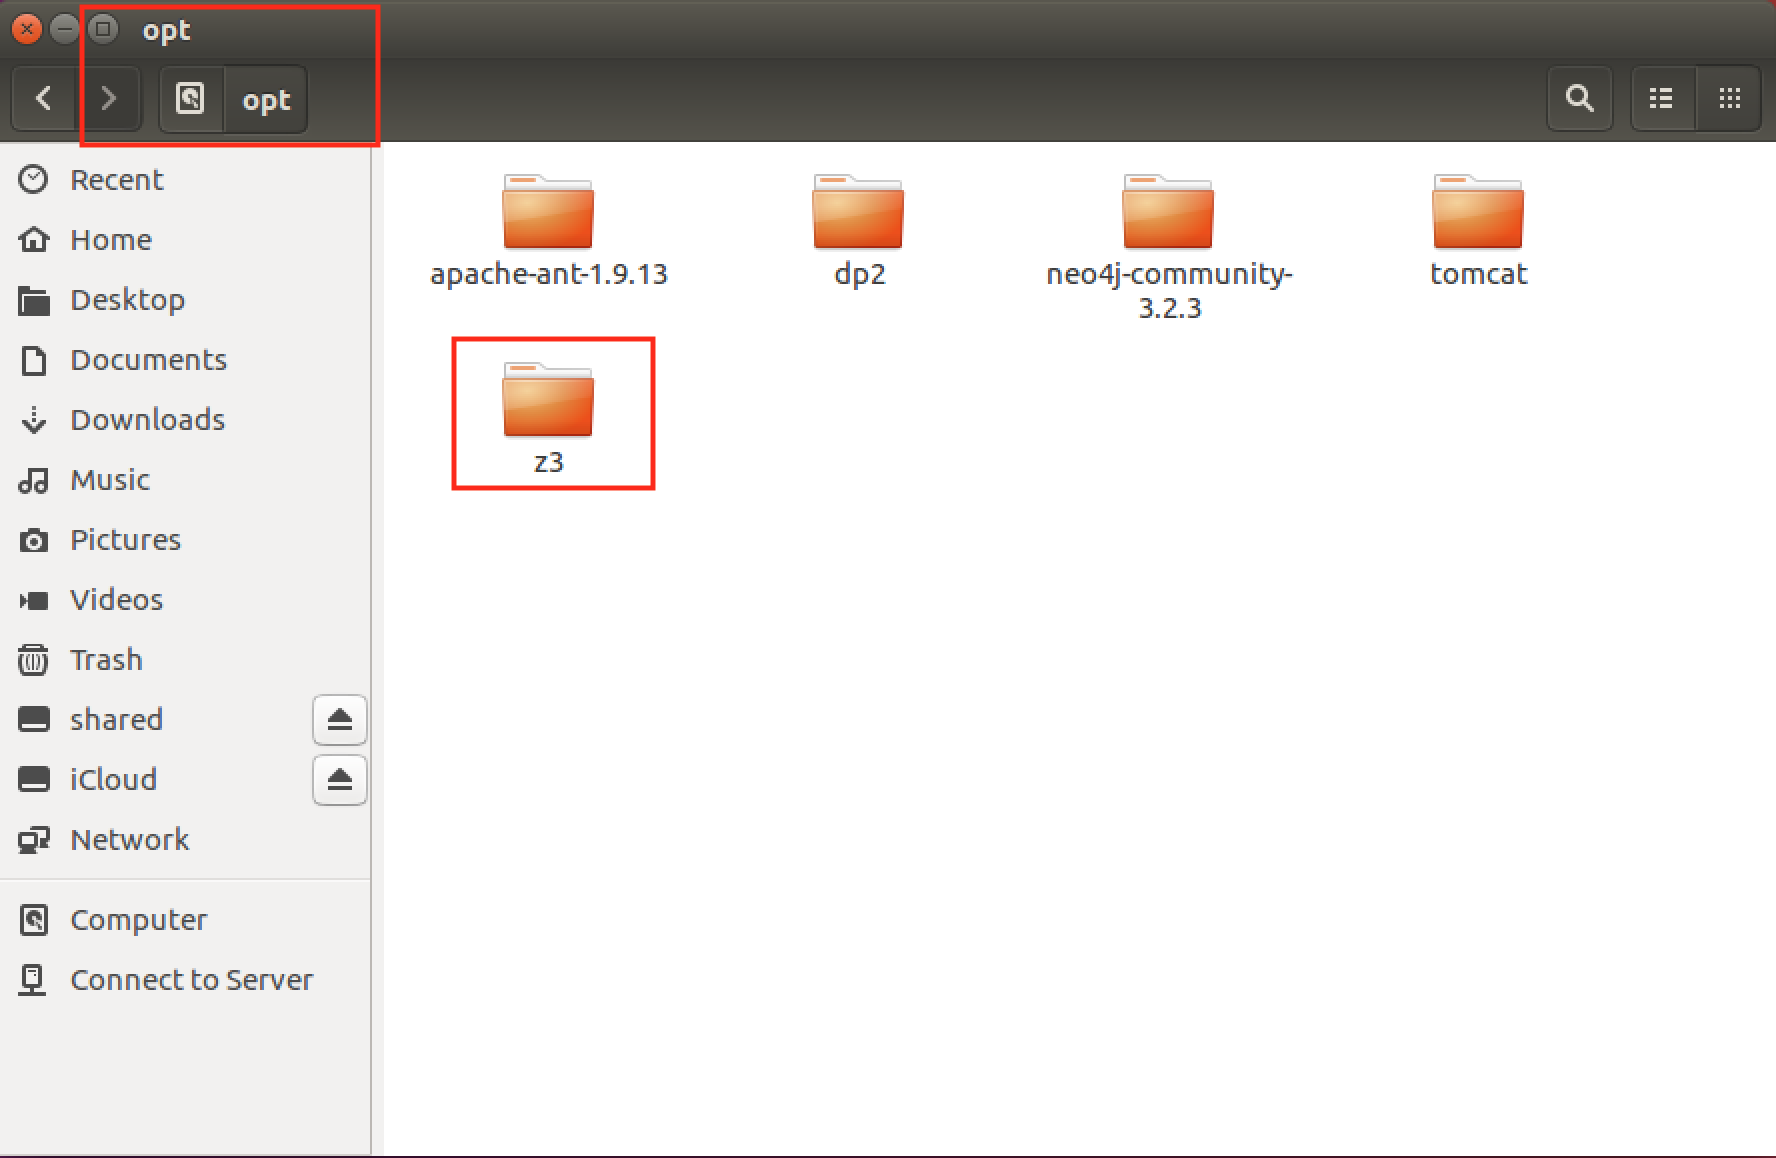
\includegraphics[width=\textwidth]{z3_location.png}
     \caption{Example of where to place Z3 extracted libraries.}\label{Fig:Z3Location}
  \end{figure}
  \item after everything has been placed in the chosen location, we have to \textbf{define} an environment variable which will allow the Java application to know where the Z3 library is located. For Ubuntu such variable is \underline{LD\_LIBRARY\_PATH}. This variable must point to the location of the \underline{bin} folder of the extracted Z3 library;
  \begin{figure}[!htb]
     \centering
     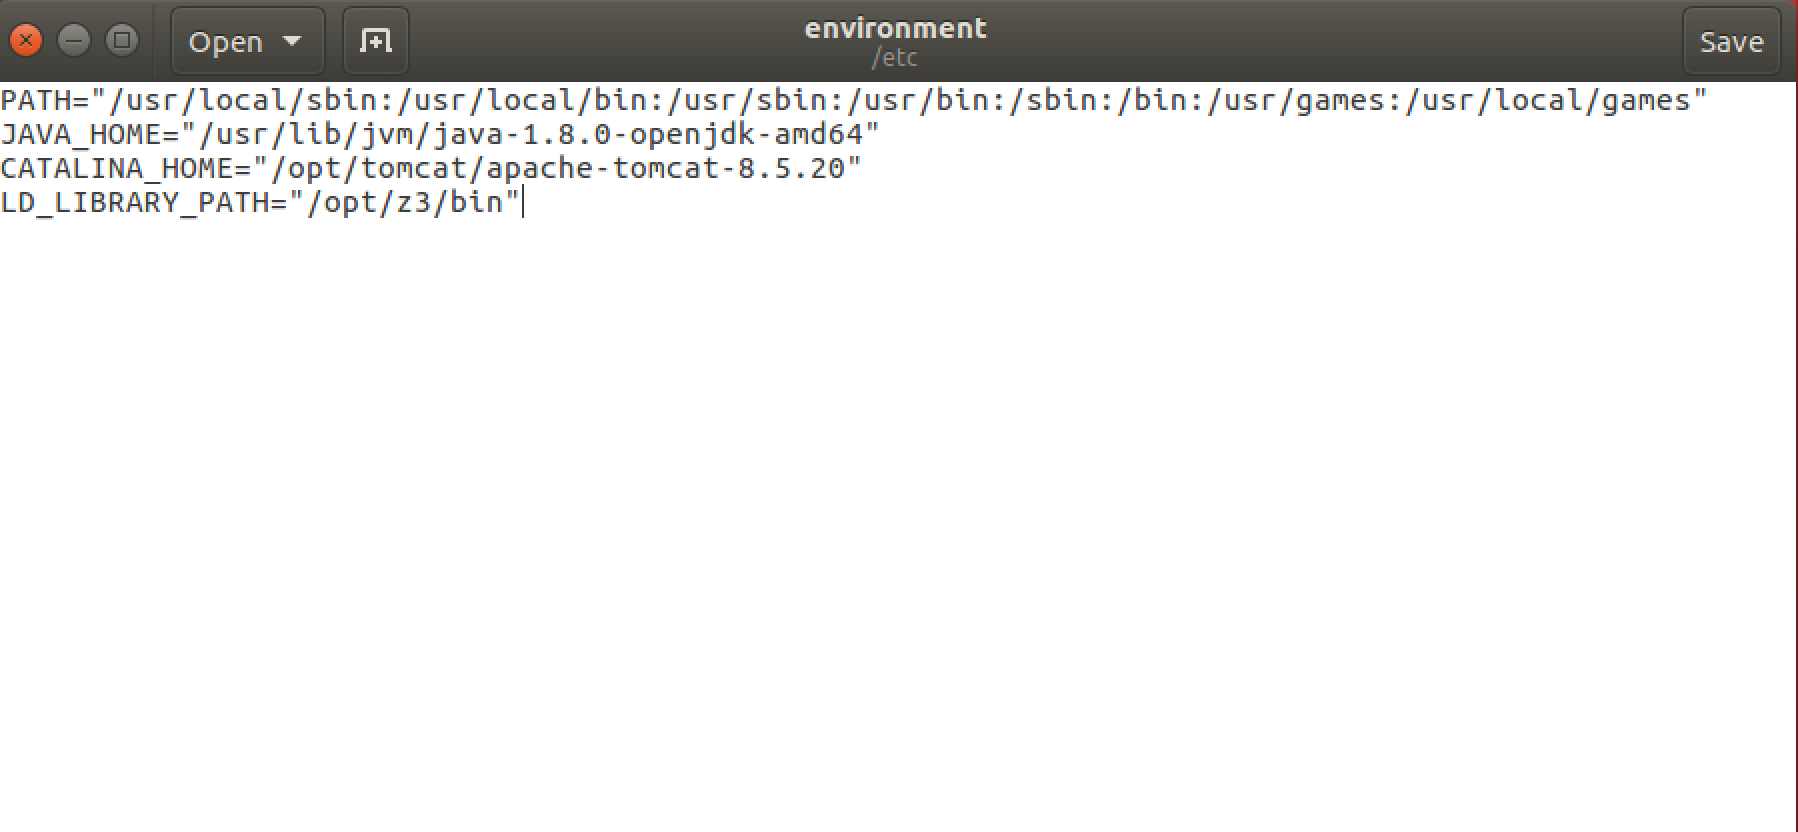
\includegraphics[width=\textwidth]{z3_environment.png}
     \caption{Example of how to define LD\_LIBRARY\_PATH environment variable.}\label{Fig:Z3Environment}
  \end{figure}
  In figure \ref{Fig:Z3Environment} is shown an example of definition of the LD\_LIBRARY\_PATH environment variable. \\
  In this case has been define globally for the whole machine, that means it has been inserted in the file \textit{/etc/environment}, but the same result could have been achieve defining it locally for the used in \textit{/Home/.bashrc} file;
  \item last step, is to add the Z3 .jar file to the build path of our project.
  \begin{figure}[!htb]
     \centering
     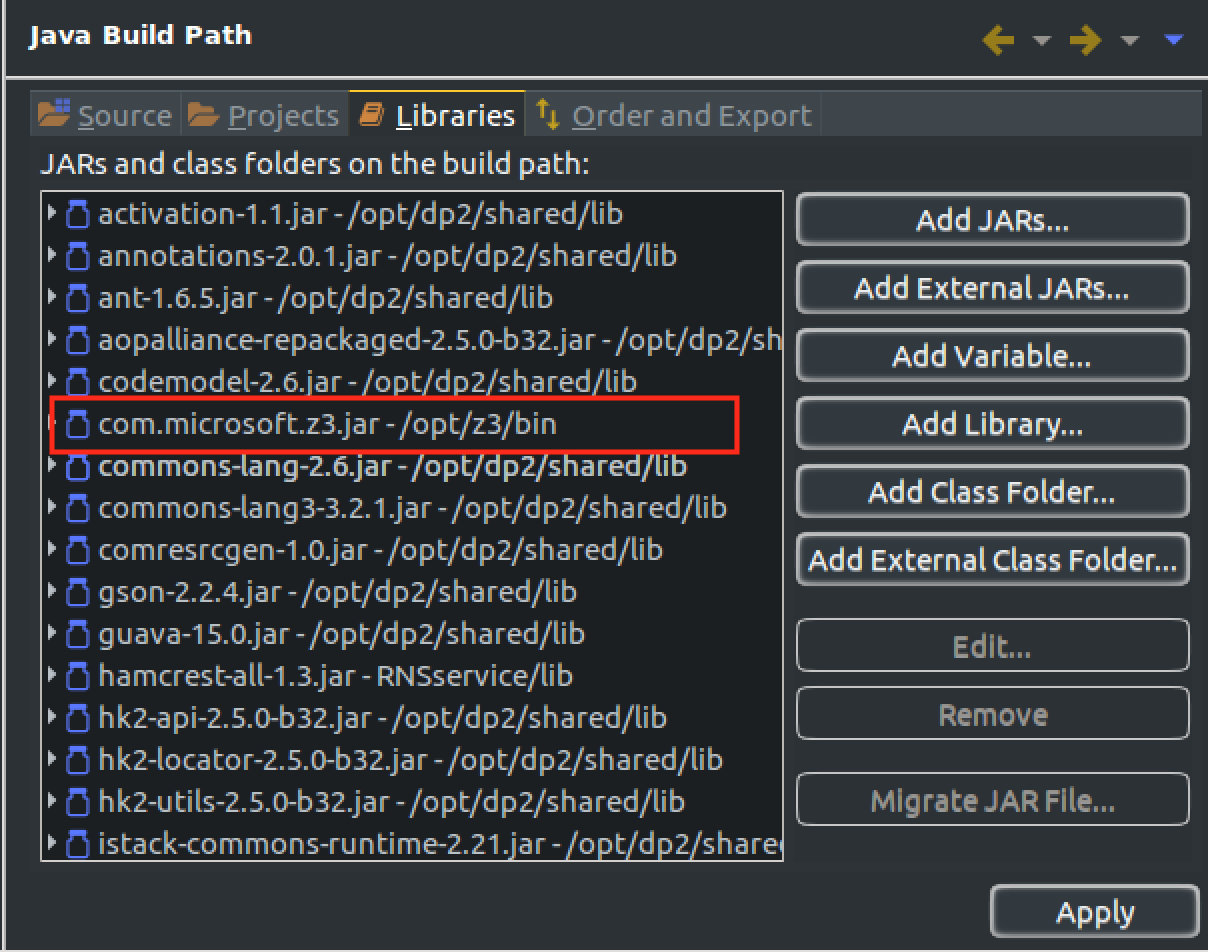
\includegraphics[width=\textwidth]{z3_buildpath.png}
     \caption{Example of how the project build path should look like.}\label{Fig:Z3BuildPath}
  \end{figure}
\end{enumerate}
This is an automatic configuration and Tomcat will load the dynamic libraries in the bin folder by itself. If this is not sufficient, we need to manually put in the WebContent/WEB-INF/lib/jni the Z3 library and point LD\_LIBRARY\_PATH to that folder.\\
Please make sure, in order to use the library in Tomcat, to have correctly set CATALINA\_HOME variable, pointing to Tomcat folder and JAVA\_HOME variable (provided you have installed Java on the machine).

% --------------------------------------------------------------------------

\subsection{Model}
In order to define a model for Z3 to work on, it has been extracted a graph from the actual map, with updated capacities and position of vehicles.\\
The criteria for a node to be selected as a possible node are:
\begin{itemize}
	\item the node doesn't contain any dangerous material.
	\item the node contains some vehicles carrying dangerous materials, but they are compatible with the one of the new vehicle.\\
\end{itemize}

\subsubsection{Mathematical Model}\label{Subs:MathModel}
The obtained mathematical model is the following.

\paragraph{Objective Function}
\begin{description}
	\item min $\ \sum_{i=1}^{N} y_{i}t_{i}$
\end{description}
\paragraph{Variables}
\begin{description}
	\item \textit{N}: number of nodes of the system
	\item $\ y_{i} \in$ \{0, 1\}: a generic node \textit{i}
	\item $\ c_{i} \geq 0$: the capacity of the node \textit{i}
	\item $\ t_{i} \in \mathbb{N}$: the weight average time spent in the node \textit{i}
	\item $\ y_{ij} \in \{0, 1\}$: a connection from node \textit{i} to node \textit{j}
\end{description}

\paragraph{Constraints}
\begin{description}
	\item $\ c_{i} \geq y_{i} $
	\item $\ \sum_{i \in N} y_{si} = 1$, where \textit{s} is the origin
	\item $\ \sum_{i \in N} y_{id} = 1$, where \textit{d} is the destination
	\item $\ \sum_{i,j \in N} y_{ij} - \sum_{i,j \in N} y_{ji} = 0$, where $\ y_{ij}$ are the incoming and $\ y_{ji}$ the outcoming connections
\end{description}

\subsubsection{Final result}
The final output of the z3 model consists in a set of boolean variables. If the value is \textbf{true}, that means that the node is to be considered in the path.\\
In the snippet \ref{Snip:Z3Model} there is an example for a path evaluated for a newly entered vehicle.
\begin{lstlisting}[frame = trBL , escapeinside={(*@}{@*)}, caption = Final result that need to be parsed to retrieve ne node ids, captionpos=b, label=Snip:Z3Model]
(define-fun y_a02-01 () Bool true)
(define-fun y_ss02 () Bool true)
(define-fun y_a02-02 () Bool false)
(define-fun y_ss01 () Bool false)
(define-fun y_a01-01 () Bool false)
(define-fun y_a01-02 () Bool true)
(define-fun y_a01-03 () Bool false)
(define-fun y_ss03 () Bool true)
(define-fun y_g05 () Bool true)
(define-fun y_g04 () Bool true)
\end{lstlisting}

% --------------------------------------------------------------------------
\subsection{Example}
In this subsection will be presented an example of how the server will compute the correct path for a new vehicle that wants to enter the system.
\begin{figure}[!htb]
   \centering
   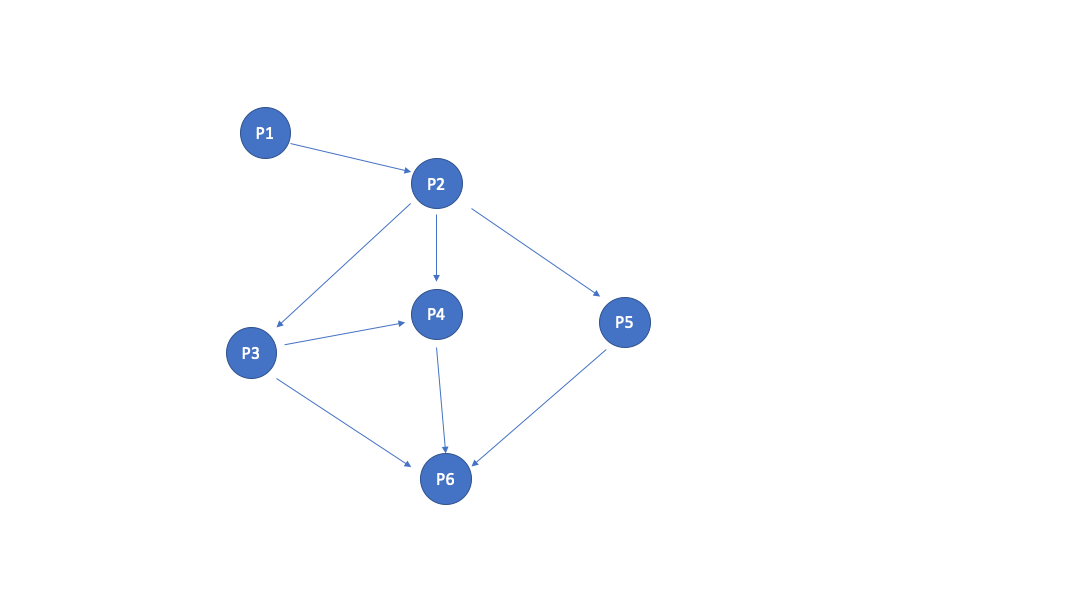
\includegraphics[width=\textwidth]{graph00.png}
   \caption{Example graph.}\label{Fig:Graph00}
\end{figure}
The initial graph that is given Z3 to work on is the one in figure \ref{Fig:Graph00}. Here two assumptions are made:
\begin{enumerate}
  \item node \textbf{P5} contains a vehicle that carries a dangerous material not compatible with the one carried by the new vehicle that wants to enter;
  \item node \textbf{P4} has not enough capacity to accept another vehicle.
\end{enumerate}
The first step that it has to be performed is selecting the origin and destination in the graph (in this case \textbf{P1} and \textbf{P6}) and infer in Z3's optimizer an hard constraint that state that both these nodes has to result \textbf{true} in order to verify the correctness of the solution. The selection of origin node (red) and destination node (green) is shown in fugire \ref{Fig:Graph01}.
\begin{figure}[!htb]
   \centering
   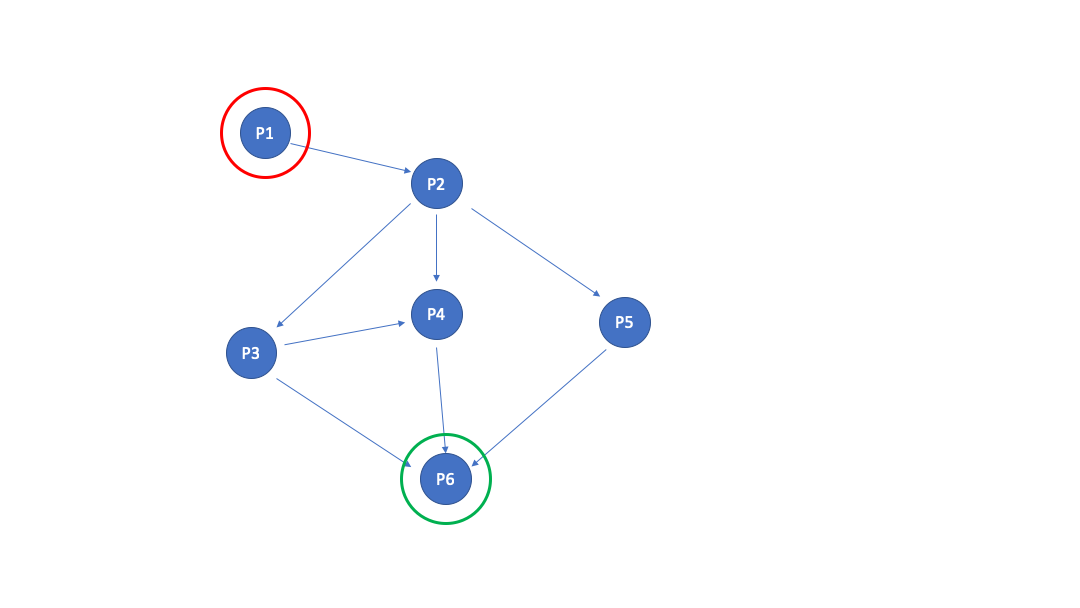
\includegraphics[width=\textwidth]{graph01.png}
   \caption{Selection of origin (red) and destination (green).}\label{Fig:Graph01}
\end{figure}
The next step is pruning from the actual graph, in order to input a correct map to Z3, all the nodes that don't meet the dangerous material constraint. Such constraint states that for a node to be selected it has not to contain any vehicle carrying materials not compatible with the one carried by the vehicle that wants to enter the system. Coherently with assumptions, node \textbf{P5} is pruned out from the graph, since it contains a vehicle with materials not compatible with the new entering (figure \ref{Fig:Graph02}).
\begin{figure}[!htb]
   \centering
   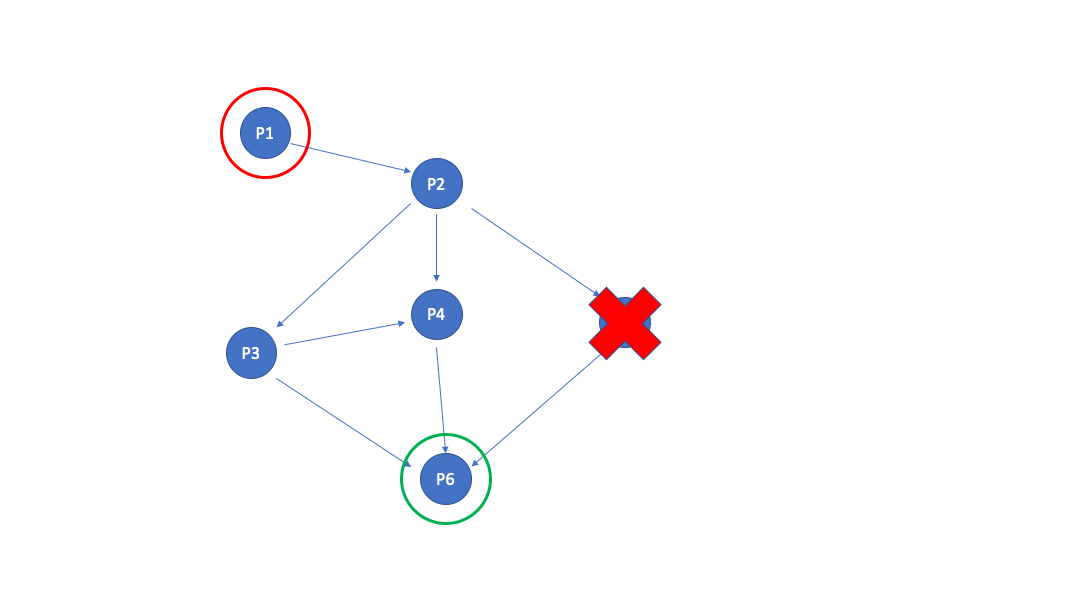
\includegraphics[width=\textwidth]{graph02.png}
   \caption{Pruning of a node due to dangerous materials constraints.}\label{Fig:Graph02}
\end{figure}
Once a correct graph has been retrieve for Z3, the next phase is to define boolean expressions for the optimizer. To achieve that, it is necessary to recur the whole graph in order to explore every node. For each one of them, different expressions has to be defined:
\begin{itemize}
  \item a boolean expression for understanding if a node is considered in the final path, that will result \textbf{true} only if one of its incoming connection's boolean expression is \textbf{true};
  \item a boolean expression for the capacity of the node, that will result to true only if the capacity of the node is greater or equal than 1. If this expression is false, it will invalidate the node as a whole, making it not suitable for the route;
  \item a boolean expression for each one the connection betwee the node and the previous ones. This is not an actual boolean expression, because it is derived from the AND between the two boolean expressions of the nodes at the end of the connection.
\end{itemize}
\begin{figure}[!htb]
   \centering
   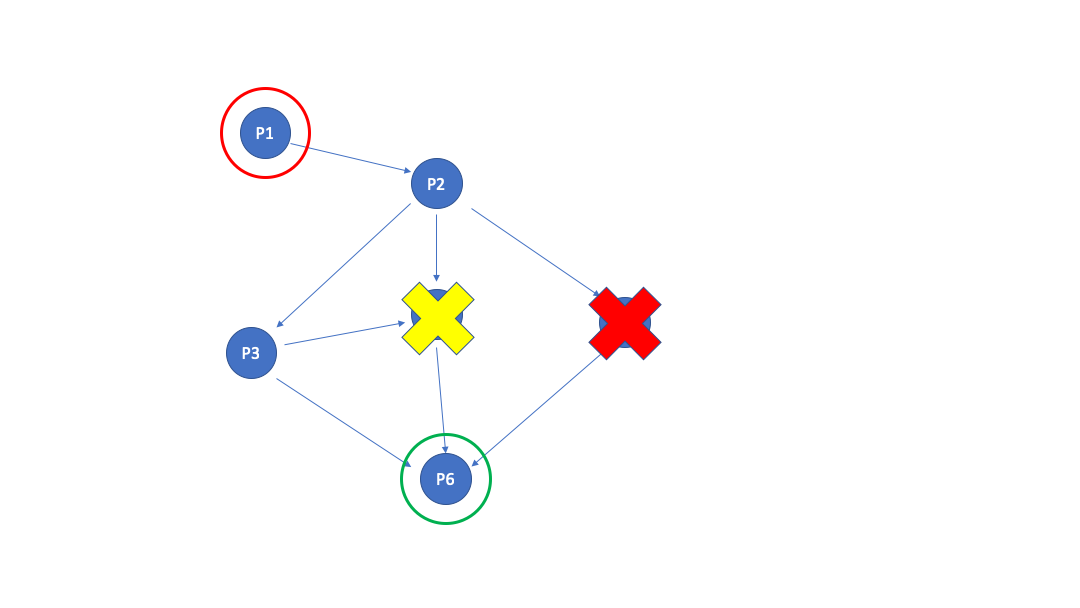
\includegraphics[width=\textwidth]{graph03.png}
   \caption{Pruning of a node due to capacity constraints.}\label{Fig:Graph03}
\end{figure}
Given the definition of such expressions, since the capacity of node \textbf{P4} doesn't meet the requirements as specified above, the corresponding boolean expression of the node is invalidated by the optimized, making it not a suitable node for the evaluation of a path as shown in figure \ref{Fig:Graph03}.
\begin{figure}[!htb]
   \centering
   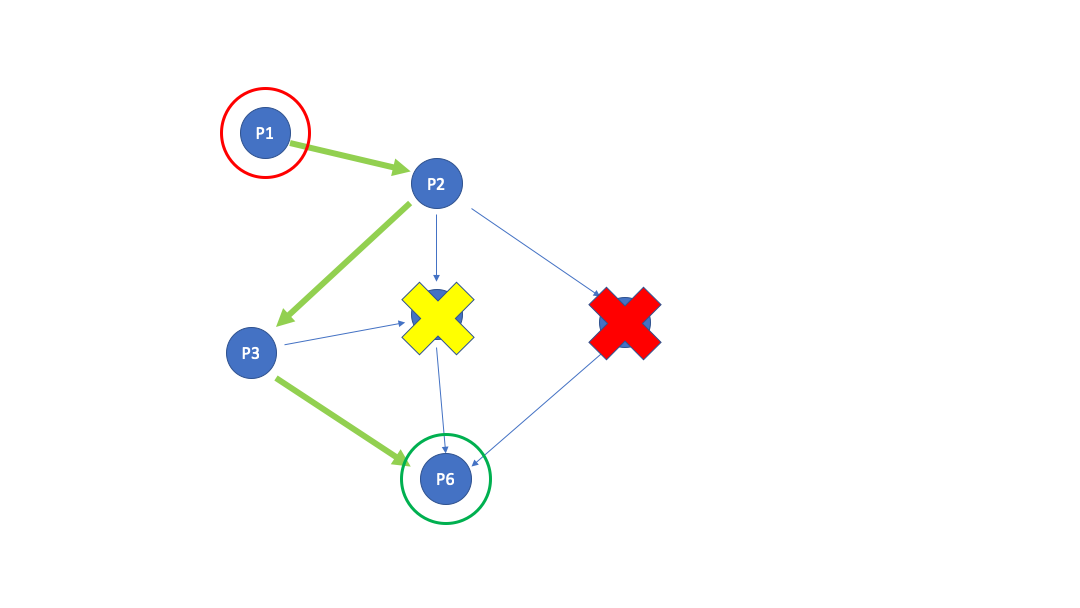
\includegraphics[width=\textwidth]{graph04.png}
   \caption{Evaluation of path from source to destination.}\label{Fig:Graph04}
\end{figure}
The resulting path produced by Z3 is the one shown in figure \ref{Fig:Graph04}. In the case multiple paths are present from source to destination, the optimizer will choose the one with the minimum traverse time, using the min time constraint define as subsection \ref{Subs:MathModel} shows.
